\chapter{Binary Classiciation at the Top}

Figure~\ref{fig: standard vs. aatp} shows the difference between the standard classifier (classifier 1) that maximizes the accuracy and the classifier that focuses only on the classification at the top (classifier 2). In this particular case, the classifier 2 tries to maximize the number of positive samples that are ranked higher than the worst negative sample, i.e. the negative sample with the highest score. Formally, we can define metric
\begin{equation*}
  \postop(\bm{s}) = \frac{1}{n^+} \sum_{i \in \I^+} \Iverson{s_i \ge \max_{i \in \I^-}\{s_i\}}.
\end{equation*}
While classifier 1 has good total~$\accuracy$, its~$\postop$ metric is subpar because of the few negative outliers. On the other hand, classifier 2 has worse total~$\accuracy$, but its~$\postop$ metric is extremely good because more than half of the positive samples are ranked higher than the worst negative sample. While classifier 1 selected different thresholds for the~$\accuracy$ and~$\postop$ metrics, these thresholds coincide for classifier 2.

\begin{figure*}
  \centering
  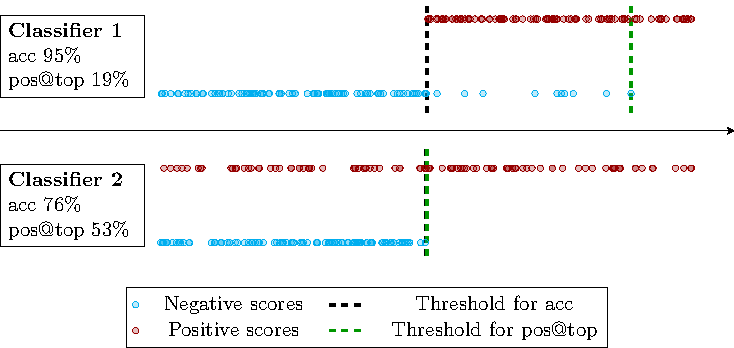
\includegraphics[width = 0.95\linewidth]{images/standard_aatp_comparison.pdf}
  \caption{Difference between standard classifiers (\textbf{Classifier~1}) and classifiers maximizing~$\postop$ metric (\textbf{Classifier~2}). While the former has a good total~$\accuracy$, the latter has a~$\postop$ metric.}
  \label{fig: standard vs. aatp}
\end{figure*}

The standard binary classification formulation~\eqref{eq: Binary classification} is not suitable for such problems because it optimizes overall performance. Moreover, all of the above examples have one thing in common: they can be formulated as a binary classification problem with special condition on the decision threshold. It means, that all these problems can be written in the following general form
\begin{mini}{\bm{w}}{
  \lambda_1 \cdot \fp(\bm{s}, t) + \lambda_2 \cdot \fn(\bm{s}, t)
}{\label{eq: aatp counts}}{}
  \addConstraint{s_i}{= f(\bm{x}_i; \bm{w}), \quad}{i = 1, 2, \ldots, n}
  \addConstraint{t}{= G(\Brac[c]{\bm{s}_i; y_i}_{i \in \I}),}
\end{mini}
where function~$G \colon\R^n \times \{0, 1\}^n \to \R$ takes the scores and labels of all samples and computes the decision threshold. The problems above only differ in the way they define the function~$G$. The important distinction from standard binary classification is that the decision threshold is no longer fixed (as in case of neural networks) or trained independently (as in case of SVM), but depends the scores of all samples.

Many important binary classification problems minimize the number of misclassified samples below (or above) certain threshold. Since these problems are usually considered separately, in this section, we provide a unified framework for their handling and present several classification problems falling into this framework. We recall the general form for binary classification at the top~\eqref{eq: aatp counts} defined in the previous chapter
\begin{mini*}{\bm{w}}{
  \lambda_1 \cdot \fp(\bm{s}, t) + \lambda_2 \cdot \fn(\bm{s}, t)
  }{}{}
  \addConstraint{s_i}{= f(\bm{x}_i; \bm{w}), \quad}{i = 1, 2, \ldots, n}
  \addConstraint{t}{= G(\Brac[c]{\bm{s}_i; y_i}_{i \in \I}).}
\end{mini*}
The objective function of the problem~\eqref{eq: aatp counts} is discontinuous because it contains Iverson function. Therefore the problem is difficult to handle. The usual approach is to employ a surrogate function such as the hinge loss or quadratic hinge loss function defined by
\begin{equation}\label{eq: hinge loss}
  \begin{aligned}
    l_{\text{hinge}}(s) & = \max\Brac[c]{0, 1 + s}.\\
    l_{\text{quadratic}}(s) & = \Brac{\max\Brac[c]{0, 1 + s}}^2.\\
  \end{aligned}
\end{equation}
In the text below, the symbol~$l$ denotes any convex non-negative non-decreasing function with~$l(0) = 1$. Using the surrogate function, the counts~\eqref{eq: confusion counts} may be approximated by their surrogate counterparts
\begin{equation}\label{eq: confusion counts surrogate}
  \begin{aligned}
    \tps(\bm{s}, t) & = \sum_{i \in \I^+}l(s_i - t), & \quad
    \fns(\bm{s}, t) & = \sum_{i \in \I^+}l(t - s_i), \\
    \tns(\bm{s}, t) & = \sum_{i \in \I^-}l(t - s_i), & \quad
    \fps(\bm{s}, t) & = \sum_{i \in \I^-}l(s_i - t).
  \end{aligned}
\end{equation}
Since~$l(\cdot)\ge[\cdot]$, the surrogate counts~\eqref{eq: confusion counts surrogate} provide upper approximations of the true counts~\eqref{eq: confusion counts}. Replacing the counts in~\eqref{eq: aatp counts}by their surrogate counterparts and adding a regularization results in
\begin{mini}{\bm{w}}{
  \frac{\lambda_0}{2}\norm{\bm{w}}^2 + \lambda_1 \cdot \fps(\bm{s}, t) + \lambda_2 \cdot \fns(\bm{s}, t)
  }{\label{eq: aatp surrogate}}{}
  \addConstraint{s_i}{= f(\bm{x}_i; \bm{w}), \quad}{i = 1, 2, \ldots, n}
  \addConstraint{t}{= G(\Brac[c]{\bm{s}_i; y_i}_{i \in \I}).}
\end{mini}
In the rest of this section, we list formulations which fall into the framework of~\eqref{eq: aatp counts} and~\eqref{eq: aatp surrogate}.


\begin{figure*}
  \centering
  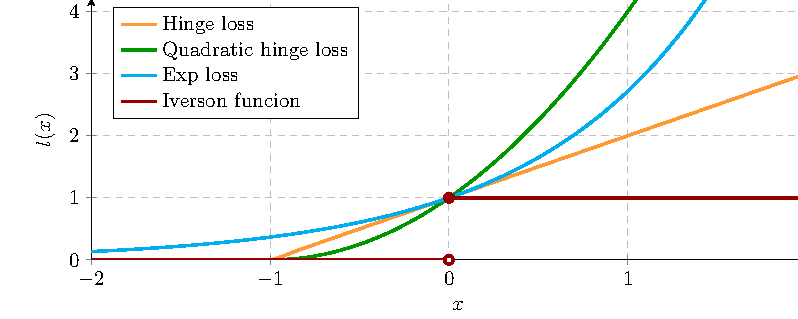
\includegraphics[width = 0.95\linewidth]{images/surrogates.pdf}
  \caption{Surrogates}
  \label{fig: surrogates}
\end{figure*}


% For samples $\bm{x}$, we consider the linear classifier $f(\bm{w}) = \bm{w}^\top \bm{x} - t$, where $\bm{w}$ is the normal vector to the separating hyperplane and $t$ is a threshold. The most well-known example is the support vector machines, where $t$ is an optimization variable. In many cases the threshold $t$ is computed from the scores $s = \bm{w}^\top \bm{x}$. For example, \TopPush from \cite{li2014top} sets the threshold $t$ to the largest score $s^-$ corresponding to negative samples and \cite{grill2016learning} sets it to the quantile of all scores.


% To be able to determine the missclassification above and below the threshold $t$, we define the true-positive, false-negative, true-negative and false-positive counts by
% \begin{equation}\label{eq: confusion counts}
%   \begin{aligned}
%     \tp(\bm{w}, t) & = \sum_{\bm{x} \in \Xc^+}\Brac[s]{\bm{w}^\top \bm{x} - t \ge 0}, &
%     \fn(\bm{w}, t) & = \sum_{\bm{x} \in \Xc^+}\Brac[s]{\bm{w}^\top \bm{x} - t < 0}, \\
%     \tn(\bm{w}, t) & = \sum_{\bm{x} \in \Xc^-}\Brac[s]{\bm{w}^\top \bm{x} - t < 0}, &
%     \fp(\bm{w}, t) & = \sum_{\bm{x} \in \Xc^-}\Brac[s]{\bm{w}^\top \bm{x} - t \ge 0}.
%   \end{aligned}
% \end{equation}
% Here $[\cdot]$ is the 0-1 loss (Iverson bracket, characteristic function) which is equal to $1$ if the argument is true and to $0$ otherwise. Moreover, $\Xc / \Xc^{+} / \Xc^{-}$ denotes the sets of all/positive/negative samples and by $n / n^{+} / n^{-}$ their respective sizes. 

% Since the misclassified samples below the threshold are the false-negatives, we arrive at the following problem
% \begin{equation}\label{eq: aatp counts}
%   \begin{aligned}
%     \minimize{}
%     & \quad \frac{1}{n^{+}}\fn(\bm{w}, t)\\
%     \st
%     & \quad \text{threshold } t \text{ is a function of }\{\bm{w}^\top \bm{x}_i\}_{i = 1}^n.
%   \end{aligned}
% \end{equation}

\section{Methods based on pushing positives to the top}\label{sec:obj1}

The first category of formulations falling into our framework~\eqref{eq: aatp counts} and~\eqref{eq: aatp surrogate} are ranking methods which attempt to put as many positives (relevant samples) to the top as possible. Specifically, for each sample $\bm{x}$, they compute the score $s = \bm{w}^\top \bm{x}$ and then sort the vector $\bm{s}$ into $\bm{s}_{[\cdot]}$ with decreasing components $s_{[1]} \ge s_{[2]} \ge \dots \ge s_{[n]}$. The number of positives on top equals to the number of positives above the highest negative. This amounts to maximizing true-positives or, equivalently, minimizing false-negatives, which may be written as
\begin{equation}\label{eq:problem_top2}
  \begin{aligned}
    \minimize{}
    & \quad\frac{1}{n^{+}}\fn(\bm{w},t) \\
    \st
    & \quad t = s_{[1]}^-, \\
    & \quad \text{components of }\bm{s}^- \text{ equal to } s^- = \bm{w}^\top \bm{x}^-\text{ for }\bm{x}^- \in \Xc^-.
  \end{aligned}
\end{equation}
As $t$ is a function of the scores $s = \bm{w}^\top \bm{x}$, problem~\eqref{eq:problem_top2} is a special case of~\eqref{eq: aatp counts}.

\TopPush from \cite{li2014top} replaces the false-negatives in~\eqref{eq:problem_top2} by their surrogate and adds a regularization term to arrive at
\begin{equation}\label{eq:problem_toppush}
  \begin{aligned}
    \minimize{}
    & \quad \frac{1}{n^{+}} \fns(\bm{w}, t) + \frac{\lambda}{2} \norm{\bm{w}}^2 \\
    \st
    & \quad t = s_{[1]}^-, \\
    & \quad \text{components of }\bm{s}^-\text{ equal to } s^- = \bm{w}^\top \bm{x}^- \text{ for }\bm{x}^- \in \Xc^-.
  \end{aligned}
\end{equation}
Note that this falls into the framework of~\eqref{eq: aatp surrogate}.

As we will show in Section \ref{sec:stability}, \TopPush is sensitive to outliers and mislabelled data. To robustify it, we follow the idea from \cite{lapin2015top} and propose to replace the largest negative score by the mean of $k$ largest negative scores. This results in
\begin{equation}\label{eq:problem_toppushk}
  \begin{aligned}
    \minimize{}
    & \quad \frac{1}{n^{+}} \fns(\bm{w}, t) + \frac{\lambda}{2} \norm{\bm{w}}^2 \\
    \st
    & \quad t = \frac{1}{k}(s_{[1]}^- + \dots + s_{[k]}^-), \\
    & \quad \text{components of } \bm{s}^- \text{ equal to } s^-= \bm{w}^\top \bm{x}^- \text{ for }\bm{x}^- \in \Xc^-.
  \end{aligned}
\end{equation}
We used the mean of highest $k$ negative scores instead of the value of the $k$-th negative score to preserve convexity as shown in Section \ref{sec:convexity}.

\section{Accuracy at the Top}\label{sec:obj2}

The previous category considers formulations which minimize the false-negatives below the highest-ranked negative. Accuracy at the Top \cite{boyd2012accuracy} takes a different approach and minimizes false-positives above the top $\tau$-quantile defined by
\begin{equation}\label{eq:defin_quantile} 
  t_1(\bm{w}) = \max \Brac[c]{t \mid \tp(\bm{w}, t) + \fp(\bm{w}, t) \ge n \tau}.
\end{equation}
Then the Accuracy at the Top problem is defined by
\begin{equation}\label{eq:problem_aatp_orig}
  \begin{aligned}
    \minimize{}
    & \quad \frac{1}{n^{-}}\fp(\bm{w},t) \\
    \st
    & \quad t \text{ is the top \ensuremath{\tau}-quantile: it solves }~\eqref{eq:defin_quantile}.
  \end{aligned}
\end{equation}
Due to Lemma \ref{lemma:fnfp_equivalence} in the Appendix, the previous problem~\eqref{eq:problem_aatp_orig} is equivalent (up to a small theoretical issue) to
\begin{equation}\label{eq:problem_aatp}
  \begin{aligned}
    \minimize{}
    & \quad \mu \fn(\bm{w}, t) + (1 - \mu)\fp(\bm{w}, t) + \frac{\lambda}{2}\norm{\bm{w}}^2\\
    \st
    & \quad t\text{ is the top \ensuremath{\tau}-quantile: it solves }\eqref{eq:defin_quantile}
  \end{aligned}
\end{equation}
for any $\mu \in [0,1]$. This problem with $\mu = 0$ equals to~\eqref{eq:problem_aatp_orig}, with $\mu = 1$ it falls into our framework~\eqref{eq: aatp counts}, while with $\mu = \frac{n^-}{n}$ it corresponds to the original definition from \cite{boyd2012accuracy}. 

Apart from the quantile~\eqref{eq:defin_quantile}, there are two other possible choices of the threshold
\begin{align}
  \label{eq:defin_quantile1} t_2(\bm{w}) =\ &\frac{1}{n\tau}\sum_{i=1}^{n\tau} s_{[i]}, \\
  \label{eq:defin_quantile0} t_3(\bm{w})\quad \text{solves} \quad & \frac{1}{n}\sum_{i = 1}^nl(\beta(s_i - t)) = \tau.
\end{align}
We again use the vector of scores $\bm{s}$ with components $s_i = \bm{w}^\top \bm{x}_i$ and for the rest of the paper we assume, for simplicity, that $n\tau$ is an integer. The quantile~\eqref{eq:defin_quantile} is sometimes denoted as VaR (value at risk) and~\eqref{eq:defin_quantile1} as CVaR (conditional value of risk). It is known is that the latter is the tightest convex approximation of the former. We will sometimes denote~\eqref{eq:defin_quantile0} as surrogate top $\tau$-quantile. We will investigate the relations between these three objects as well as their properties such as convexity, differentiability or stability in Section \ref{sec:theory}.

Paper \cite{grill2016learning} builds on the Accuracy at the Top problem~\eqref{eq:problem_aatp}, where it replaces $\fn(\bm{w}, t)$ and $\fp(\bm{w}, t)$ in the objective by their surrogate counterparts $\fns(\bm{w}, t)$ and $\fps(\bm{w}, t)$. This leads to
\begin{equation}\label{eq:problem_grill}
  \begin{aligned}
    \minimize{}
    & \quad \frac{1}{n^{+}}\fns(\bm{w},t) + \frac{1}{n^{-}}\fps(\bm{w},t) + \frac{\lambda}{2}\norm{\bm{w}}^2\\
    \st
    & \quad t\text{ is the top \ensuremath{\tau}-quantile: it solves }\eqref{eq:defin_quantile}.
  \end{aligned}
\end{equation}
Based on the first author, we name this formulation \Grill. The main purpose of~\eqref{eq:defin_quantile1} is to provide a convex approximation of the non-convex quantile~\eqref{eq:defin_quantile}. Putting it into the constraint results in a convex approximation problem, which we call \TopMeanK
\begin{equation}\label{eq:problem_topmeank}
  \begin{aligned}
    \minimize{}
    & \quad \frac{1}{n^{+}} \fns(\bm{w},t) + \frac{\lambda}{2}\norm{\bm{w}}^2 \\
    \st
    & \quad t = \frac 1{n\tau}(s_{[1]} + \dots + s_{[n\tau]}), \\
    & \quad \text{components of }\bm{s}\text{ equal to } s = \bm{w}^\top \bm{x} \text{ for } \bm{x} \in \Xc.
  \end{aligned}
\end{equation}
Similarly, we can use the surrogate top quantile in the constraint to arrive at
\begin{equation}\label{eq:problem_patmat}
  \begin{aligned}
    \minimize{}
    & \quad \frac{1}{n^{+}} \fns(\bm{w},t) + \frac{\lambda}{2}\norm{\bm{w}}^2\\
    \st
    & \quad t \text{ is the surrogate top \ensuremath{\tau}-quantile: it solves }\eqref{eq:defin_quantile0}.
  \end{aligned}
\end{equation}
Note that \Grill minimizes the convex combination of false-positives and false-negatives while~\eqref{eq:problem_topmeank} and~\eqref{eq:problem_patmat} minimize only the false-negatives. The reason for this will be evident in Section \ref{sec:convexity} and amounts to preservation of convexity. Moreover, as will see later, problem~\eqref{eq:problem_patmat} provides a good approximation to the Accuracy at the Top problem, it is easily solvable due to convexity and requires almost no tuning, we named it \PatMat (Precision At the Top \& Mostly Automated Tuning). 

\section{Methods optimizing the Neyman-Pearson criterion}\label{sec:obj3}

Another category falling into the framework of~\eqref{eq: aatp counts} and~\eqref{eq: aatp surrogate} is the Neyman-Pearson problem which is closely related to hypothesis testing, where null $H_0$ and alternative $H_1$ hypotheses are given. Type~I error occurs when $H_0$ is true but is rejected, and type II error happens when $H_0$ is false, but it fails to be rejected. The standard technique is to minimize Type II error while a bound for Type I error is given.

In the Neyman-Pearson problem, the null hypothesis $H_0$ states that a sample $\bm{x}$ has the negative label. Then Type I error corresponds to false-positives while Type II error to false-negatives. If the bound on Type I error equals $\tau$, we may write this as
\begin{equation}\label{eq:defin_quantile_np} 
  t_1^{\rm NP}(\bm{w}) = \max\Brac[c]{t \mid \fp(\bm{w},t) \ge n^- \tau}.
\end{equation}
Then, we may write the Neyman-Pearson problem as
\begin{equation}\label{eq:problem_np}
  \begin{aligned}
    \minimize{}
    & \quad \frac{1}{n^{+}}\fn(\bm{w},t) \\
    \st
    & \quad t \text{ is Type I error at level \ensuremath{\tau}: it solves }\eqref{eq:defin_quantile_np}.
  \end{aligned}
\end{equation}
Since~\eqref{eq:problem_np} differs from~\eqref{eq:problem_aatp} only by counting only the false-positives in~\eqref{eq:defin_quantile_np} instead of counting all positives in~\eqref{eq:defin_quantile}, we can derive its approximations in exactly the same way as in Section \ref{sec:obj2}. We therefore provide only their brief description and start with approximations of~\eqref{eq:defin_quantile_np}
\begin{align}
  \label{eq:defin_quantile1_np} t_2^{\rm NP}(\bm{w}) =\ &\frac{1}{n^-\tau}\sum_{i=1}^{n^-\tau} s_{[i]}^-, \\
  \label{eq:defin_quantile0_np} t_3^{\rm NP}(\bm{w})\quad \text{solves} \quad &\frac{1}{n}\sum_{i=1}^{n^-}l(\beta(s_i^- - t)) = \tau.
\end{align}
Replacing the true counts by their surrogates results in the Neyman-Pearson variant \GrillNP
\begin{equation}\label{eq:problem_grill_np}
  \begin{aligned}
  \minimize{}
  & \quad \frac{1}{n^{+}}\fns(\bm{w}, t) + \frac{1}{n^{-}}\fps(\bm{w}, t) + \frac{\lambda}{2}\norm{\bm{w}}^2\\
  \st
  & \quad t\text{ is the Neyman-Pearson threshold: it solves }\eqref{eq:defin_quantile_np}.
  \end{aligned}
\end{equation}
Similarly, the Neyman-Pearson alternative to \TopMeanK reads
\begin{equation}\label{eq:problem_topmeank_np}
  \begin{aligned}
  \minimize{}
  & \quad\frac{1}{n^{+}}\fns(\bm{w}, t) + \frac{\lambda}{2}\norm{\bm{w}}^2 \\
  \st
  & \quad t = \frac 1{n^ - \tau}(s_{[1]}^- + \dots + s_{[n^- \tau]}^-), \\
  & \quad \text{components of }\bm{s}^-\text{ equal to } s^- = \bm{w}^\top \bm{x}^-\text{ for }\bm{x}^- \in \Xc.
  \end{aligned}
\end{equation}
This problem already appeared in \cite{zhang2018tau} under the name \tauFPL. Finally, \PatMatNP reads
\begin{equation}\label{eq:problem_patmat_np}
  \begin{aligned}
  \minimize{}
  & \quad \frac{1}{n^{+}}\fns(\bm{w},t) + \frac{\lambda}{2}\norm{\bm{w}}^2\\
  \st
  & \quad t\text{ is the surrogate Neyman-Pearson threshold: it solves }\eqref{eq:defin_quantile0_np}.
  \end{aligned}
\end{equation}

We may see~\eqref{eq:problem_topmeank_np} from two different viewpoints. First, \tauFPL provide convex approximations of \GrillNP. Second, \tauFPL has the same form as \TopPushK. The only difference is that for \tauFPL we have $k=n^-\tau$ while for \TopPushK the value of $k$ is small. Thus, even though we started from two different problems, we arrived at two approximations which differ only in the value of one parameter. This shows a close relation of the ranking problem and the Neyman-Pearson problem and the need for a unified theory to handle these problems.
